\documentclass{beamer}
\usepackage[latin1]{inputenc}
\usepackage{times}
\usepackage{tikz}
\usetheme{Luebeck}
%\usecolortheme{albatross}
\usepackage{amsmath,amsfonts,amsthm,amssymb}
\usepackage{setspace}
\usepackage{Tabbing}
\usepackage{fancyhdr}
\usepackage{lastpage}
\usepackage{extramarks}
\usepackage{chngpage}
\usepackage{soul,color}
\usepackage{graphicx,float,wrapfig}
\usepackage{xcolor}
\usepackage{listings}
\usepackage{float}
%\usepackage{subfloat}
\usepackage{subfig}
\usepackage{caption}
\usepackage{enumitem}
\usepackage{algpseudocode}

\definecolor{darkorange}{RGB}{240, 120, 0}
\definecolor{darkgreen}{RGB}{0, 128, 0}

\setbeamercolor{background canvas}{bg=white}
\setbeamercolor{frametitle}{fg=white, bg=darkorange}
\setbeamercolor{normal text}{bg=black,fg=black}
\setbeamercolor{structure}{bg=black, fg=darkorange}

\title{Lecture 10: Point Clouds, Eigenvectors, PCA}
\date{2/16/2016}
\institute{Chris Tralie, Duke University}
\author{COMPSCI/MATH 290-04}
\begin{document}

\frame{\titlepage}

\begin{frame}{Announcements}

\begin{itemize}[label=$\blacktriangleright$]
    \item Group Assignment 1 Part 1, Due This Sunday 11:55 PM
    \item Note on Assignment Difficulty
    \item Hackathon 2/26, 2/27, or 2/28 (upcoming poll)
    \item Choosing final projects before spring break
    \item Visitors Coming...
\end{itemize}

\end{frame}

\begin{frame}{Table of Contents}

\begin{itemize}[label=$\blacktriangleright$]
	\item Point Clouds Unit Overview
\end{itemize}
\begin{itemize}[label=$\vartriangleright$]
	\item Eigenvalues / Eigenvectors
	\item Principal Component Analysis
\end{itemize}

\end{frame}

\begin{frame}{What Is A Point Cloud?}

Interactive Demo

\end{frame}


\begin{frame}{What's In This Unit?}
Point Cloud Registration (Alignment)

\begin{figure}[t]
    \centering
	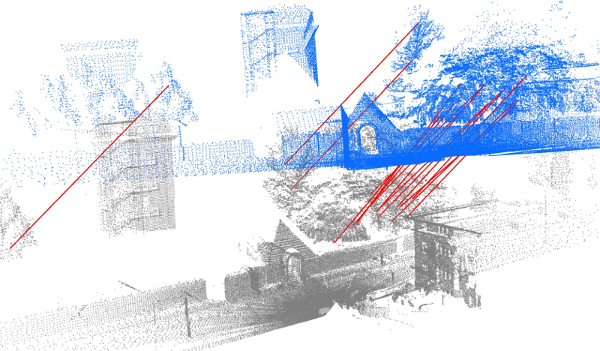
\includegraphics[width=0.9\textwidth]{registration_outdoor_pcl.png}
\end{figure}

Courtesy of \url{http://www.pointclouds.org}

\end{frame}

\begin{frame}{What's In This Unit?}
``Shape Google" (Point Cloud Statistics)

\begin{figure}[t]
    \centering
	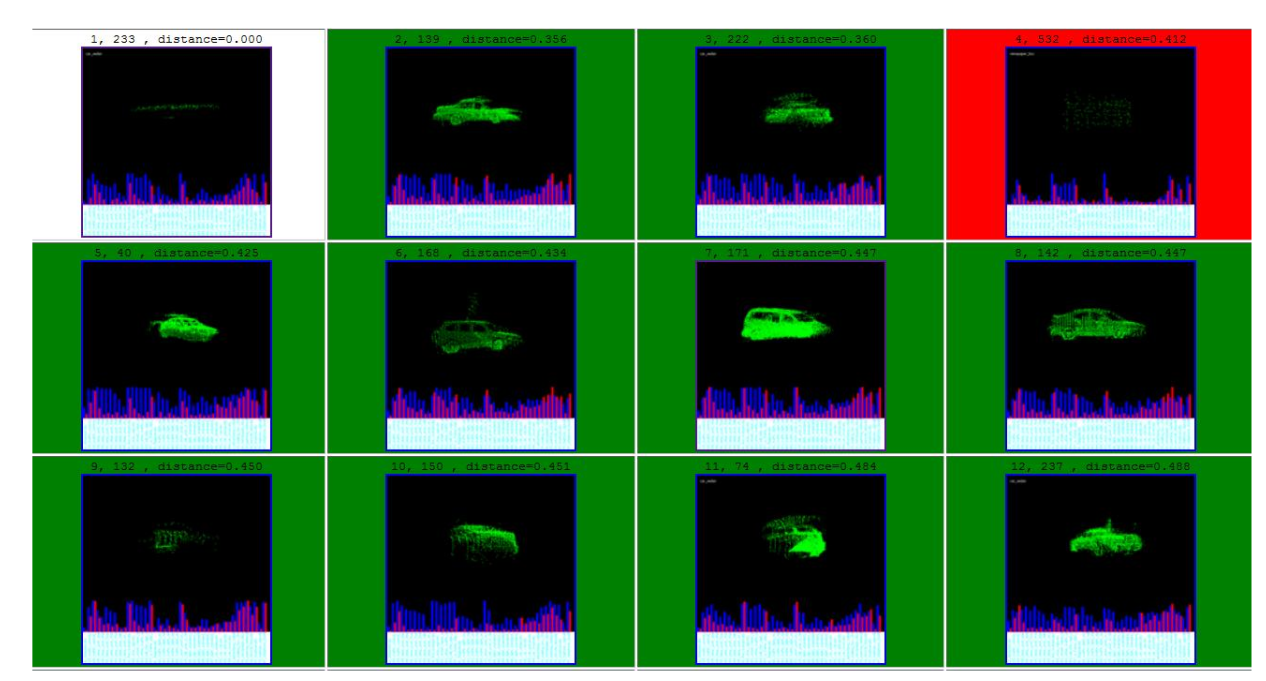
\includegraphics[width=0.9\textwidth]{ShapeGoogle.png}
\end{figure}

(my undergrad senior thesis)

\end{frame}

\begin{frame}{What's In This Unit?}
Symmetries

\begin{figure}[t]
    \centering
	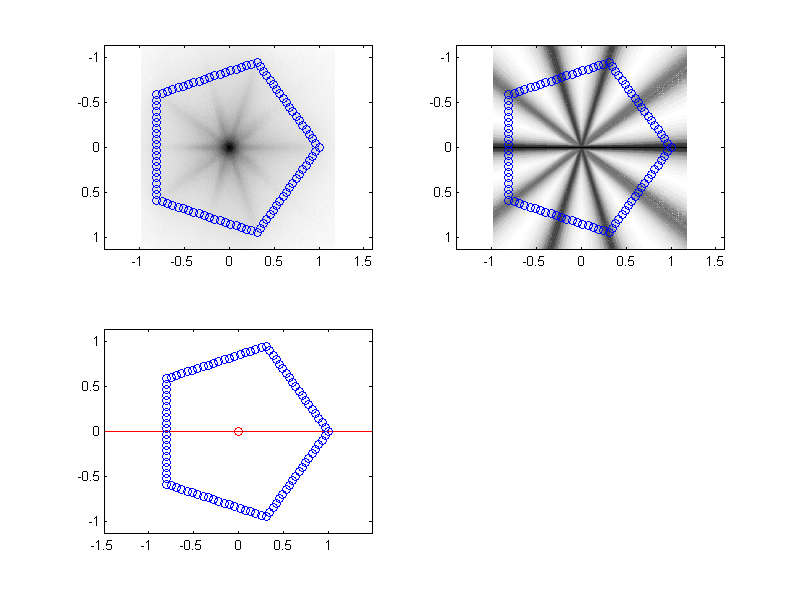
\includegraphics[width=0.9\textwidth]{pentagonsym.png}
\end{figure}

\end{frame}

\begin{frame}{What's In This Unit?}
Symmetries

\begin{figure}[t]
    \centering
	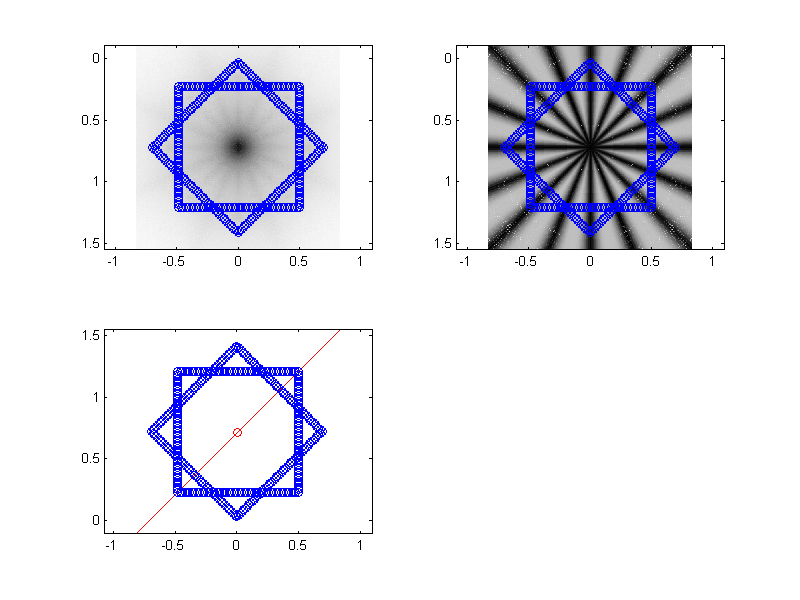
\includegraphics[width=0.9\textwidth]{starsym.png}
\end{figure}

\end{frame}

\begin{frame}{What's In This Unit?}
Symmetries

\begin{figure}[t]
    \centering
	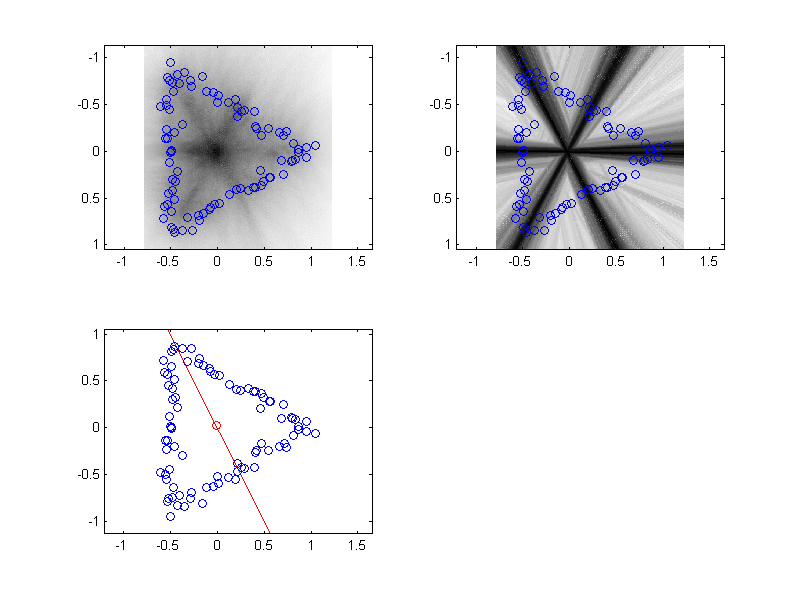
\includegraphics[width=0.9\textwidth]{trianglesym1.png}
\end{figure}

\end{frame}


\begin{frame}{What's In This Unit?}
Surface Reconstruction
\begin{figure}[t]
    \centering
	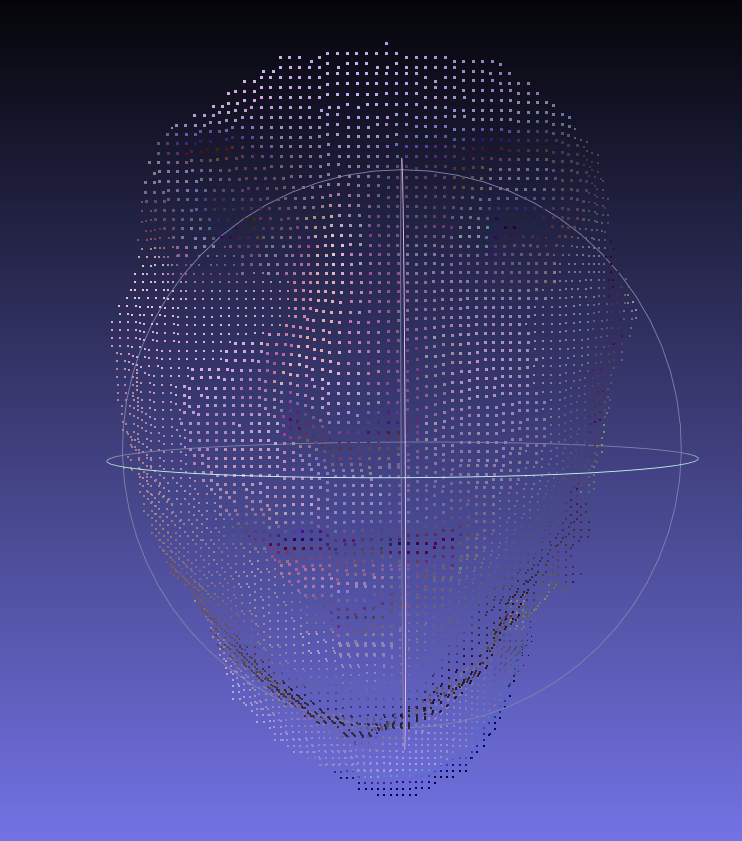
\includegraphics[width=0.5\textwidth]{PCOriginal.png}
\end{figure}

\end{frame}

\begin{frame}{What's In This Unit?}
Surface Reconstruction
\begin{figure}[t]
    \centering
	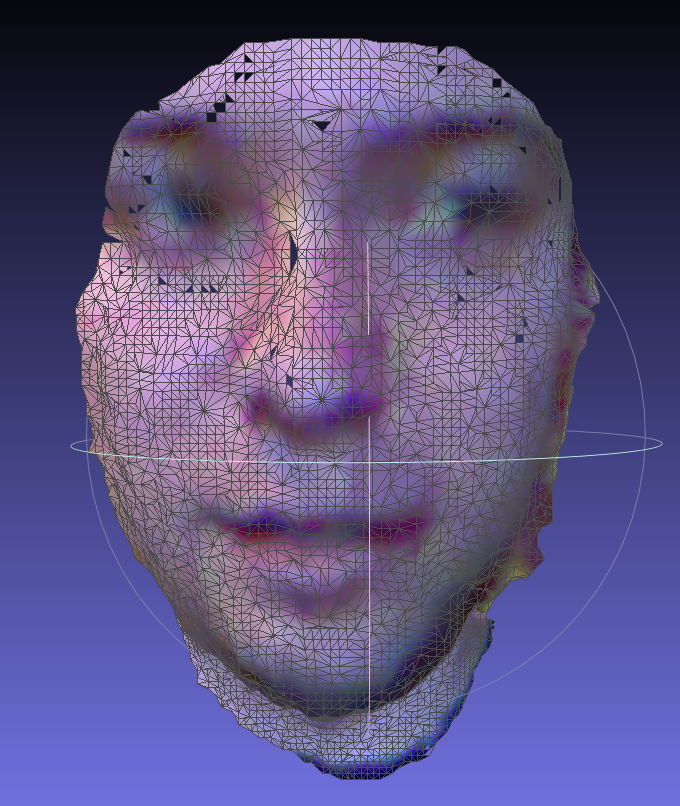
\includegraphics[width=0.5\textwidth]{PCReconstructed.png}
\end{figure}

\end{frame}



\begin{frame}{Table of Contents}

\begin{itemize}[label=$\vartriangleright$]
	\item Point Clouds Unit Overview
\end{itemize}
\begin{itemize}[label=$\blacktriangleright$]
	\item Eigenvalues / Eigenvectors
\end{itemize}
\begin{itemize}[label=$\vartriangleright$]
	\item Principal Component Analysis
\end{itemize}

\end{frame}


\begin{frame}{Eigenvalues/Eigenvectors}

\[ Ax = \lambda x \]

$A$ is $N \times N$ matrix

$x$ is $N \times 1$ column matrix (vector)

$\lambda$ is a scalar called the {\em eigenvalue} of $x$


\uncover<2->{
\begin{itemize}[label=$\vartriangleright$]
\item $A$ does not change the direction of $x$
\end{itemize}
}


\end{frame}


\begin{frame}{Eigenvalues/Eigenvectors Example: X Scale}

\only<1>{
\[ \left[ \begin{array}{cc} 2 & 0\\ 0 & 1 \end{array} \right] \left[ \begin{array}{c} 0 \\ 1 \end{array} \right] =   \]
}
\only<2>{
\[ \left[ \begin{array}{cc} 2 & 0\\ 0 & 1 \end{array} \right] \left[ \begin{array}{c} 0 \\ 1 \end{array} \right] =  \left[ \begin{array}{c} 0 \\ 1 \end{array} \right] \]
}

\only<2>{
Yes!  $\lambda = 1$
}

\begin{figure}[t]
    \captionsetup[subfloat]{labelformat=empty}
	\centering
	\subfloat[Before]{
	    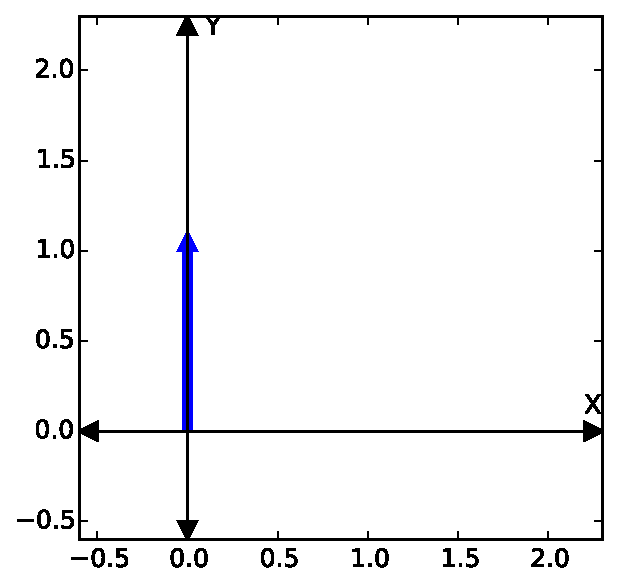
\includegraphics[width=0.46\textwidth]{2DScaleXEig2.pdf}
	}
	\uncover<2->{
	\subfloat[After]{
	    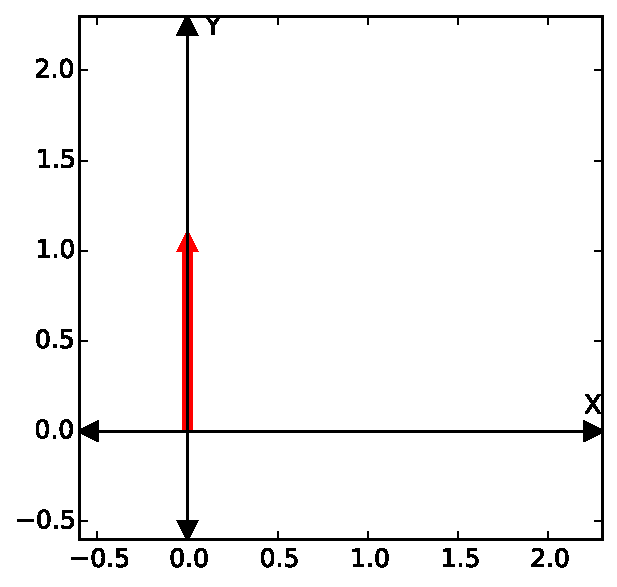
\includegraphics[width=0.46\textwidth]{2DScaleXEig2_T.pdf}
	}
	}
\end{figure}

\end{frame}



\begin{frame}{Eigenvalues/Eigenvectors Example: X Scale}

\only<1>{
\[ \left[ \begin{array}{cc} 2 & 0\\ 0 & 1 \end{array} \right] \left[ \begin{array}{c} 1 \\ 0 \end{array} \right] =   \]
}
\only<2>{
\[ \left[ \begin{array}{cc} 2 & 0\\ 0 & 1 \end{array} \right] \left[ \begin{array}{c} 1 \\ 0 \end{array} \right] =  \left[ \begin{array}{c} 2 \\ 0 \end{array} \right] \]
}

\only<2>{
Yes!  $\lambda = 2$
}

\begin{figure}[t]
    \captionsetup[subfloat]{labelformat=empty}
	\centering
	\subfloat[Before]{
	    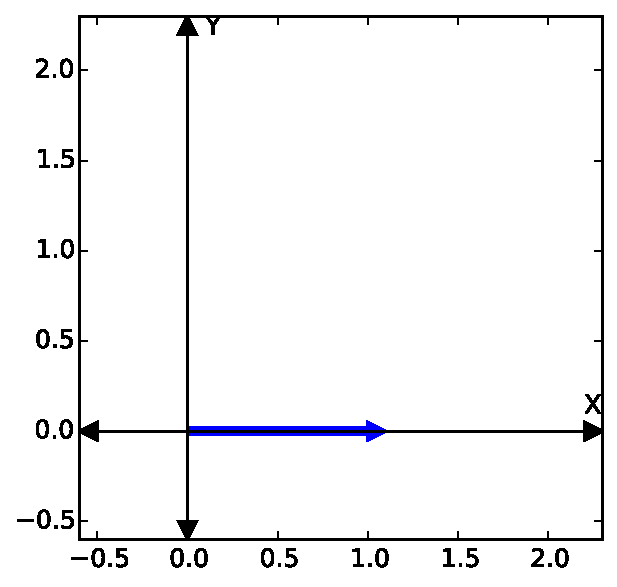
\includegraphics[width=0.46\textwidth]{2DScaleXEig1.pdf}
	}
	\uncover<2->{
	\subfloat[After]{
	    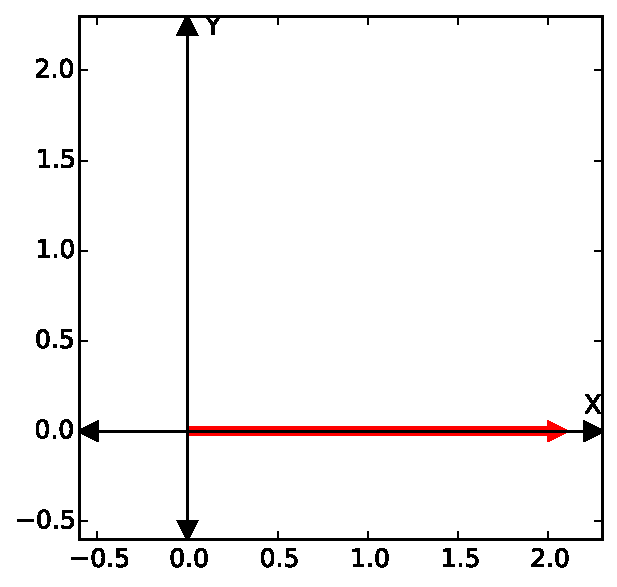
\includegraphics[width=0.46\textwidth]{2DScaleXEig1_T.pdf}
	}
	}
\end{figure}

\end{frame}


\begin{frame}{Eigenvalues/Eigenvectors Example: X Scale}

\only<1>{
\[ \left[ \begin{array}{cc} 2 & 0\\ 0 & 1 \end{array} \right] \left[ \begin{array}{c} 1 \\ 1 \end{array} \right] =   \]
}
\only<2>{
\[ \left[ \begin{array}{cc} 2 & 0\\ 0 & 1 \end{array} \right] \left[ \begin{array}{c} 1 \\ 1 \end{array} \right] =  \left[ \begin{array}{c} 2 \\ 1 \end{array} \right] \]
}

\only<2>{
No, changes direction
}

\begin{figure}[t]
    \captionsetup[subfloat]{labelformat=empty}
	\centering
	\subfloat[Before]{
	    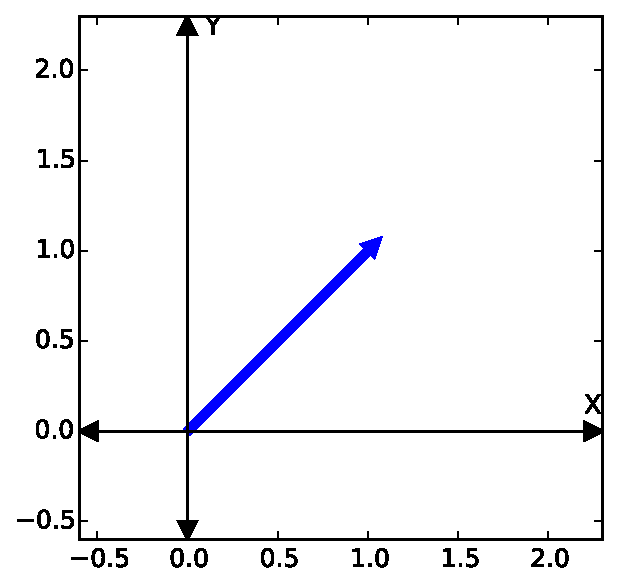
\includegraphics[width=0.46\textwidth]{2DScaleXEig3.pdf}
	}
	\uncover<2->{
	\subfloat[After]{
	    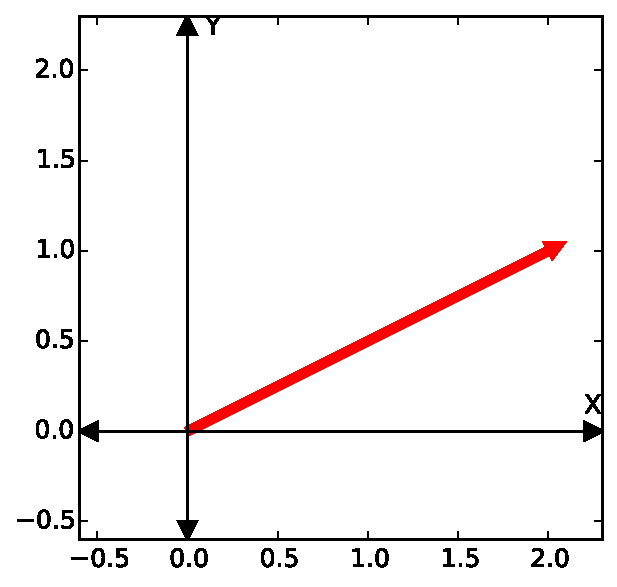
\includegraphics[width=0.46\textwidth]{2DScaleXEig3_T.pdf}
	}
	}
\end{figure}

\end{frame}

\begin{frame}{Eigenvalues/Eigenvectors Example: Shear}

\only<1>{
\[ \left[ \begin{array}{cc} 1 & 1\\ 0 & 1 \end{array} \right] \left[ \begin{array}{c} 1 \\ 0 \end{array} \right] =   \]
}
\only<2>{
\[ \left[ \begin{array}{cc} 1 & 1\\ 0 & 1 \end{array} \right] \left[ \begin{array}{c} 1 \\ 0 \end{array} \right] =  \left[ \begin{array}{c} 1 \\ 0 \end{array} \right] \]
}

\only<2>{
Yes!  $\lambda = 1$
}

\begin{figure}[t]
    \captionsetup[subfloat]{labelformat=empty}
	\centering
	\subfloat[Before]{
	    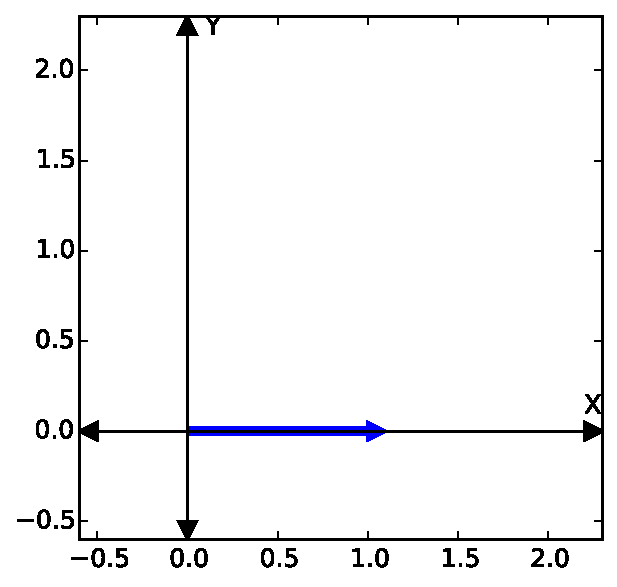
\includegraphics[width=0.46\textwidth]{2DShearXEig1.pdf}
	}
	\uncover<2->{
	\subfloat[After]{
	    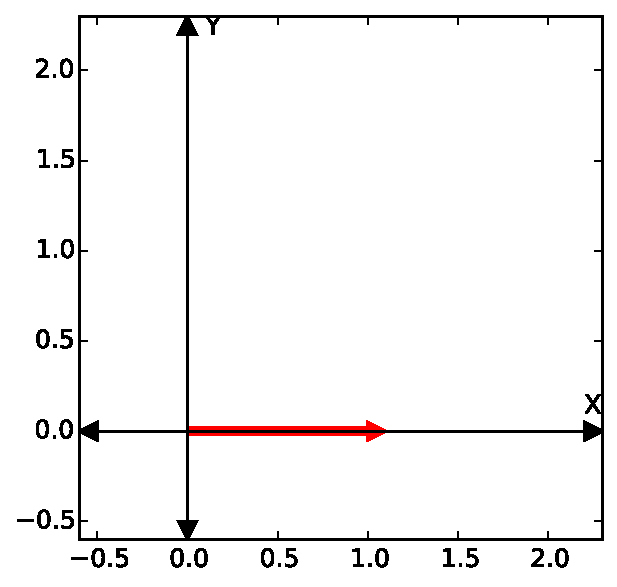
\includegraphics[width=0.46\textwidth]{2DShearXEig1_T.pdf}
	}
	}
\end{figure}



\end{frame}


\begin{frame}{Eigenvalues/Eigenvectors Example: Shear}

\only<1>{
\[ \left[ \begin{array}{cc} 1 & 1\\ 0 & 1 \end{array} \right] \left[ \begin{array}{c} 0 \\ 1 \end{array} \right] =   \]
}
\only<2>{
\[ \left[ \begin{array}{cc} 1 & 1\\ 0 & 1 \end{array} \right] \left[ \begin{array}{c} 0 \\ 1 \end{array} \right] =  \left[ \begin{array}{c} 1 \\ 1 \end{array} \right] \]
}

\only<2>{
No, changes direction
}

\begin{figure}[t]
    \captionsetup[subfloat]{labelformat=empty}
	\centering
	\subfloat[Before]{
	    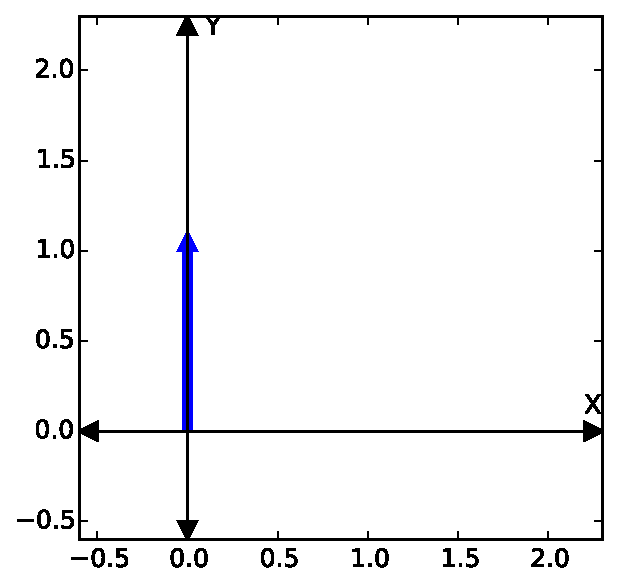
\includegraphics[width=0.46\textwidth]{2DShearXEig2.pdf}
	}
	\uncover<2->{
	\subfloat[After]{
	    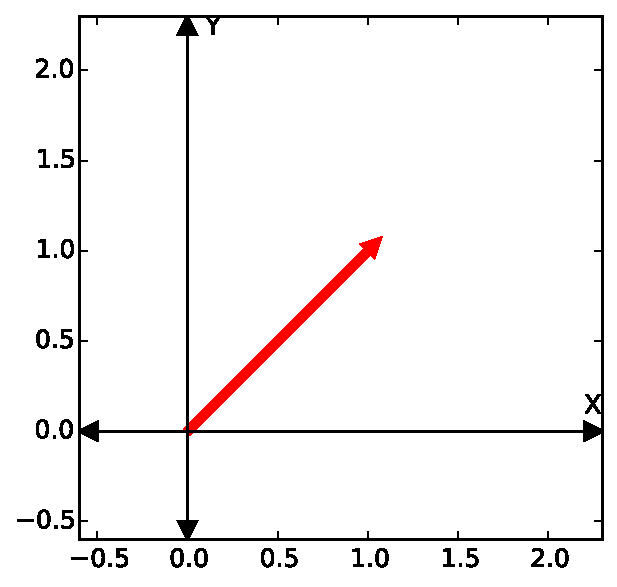
\includegraphics[width=0.46\textwidth]{2DShearXEig2_T.pdf}
	}
	}
\end{figure}



\end{frame}

\begin{frame}{Eigenvalues/Eigenvectors Example: Flip X, Scale Y}

\only<1>{
\[ \left[ \begin{array}{cc} -1 & 0\\ 0 & 2 \end{array} \right] \left[ \begin{array}{c} 1 \\ 0 \end{array} \right] =   \]
}
\only<2>{
\[ \left[ \begin{array}{cc} -1 & 0\\ 0 & 2 \end{array} \right] \left[ \begin{array}{c} 1 \\ 0 \end{array} \right] =  \left[ \begin{array}{c} -1 \\ 0 \end{array} \right] \]
}

\only<2>{
Yes!  $\lambda = -1$ (tricky)
}


\begin{figure}[t]
    \captionsetup[subfloat]{labelformat=empty}
	\centering
	\subfloat[Before]{
	    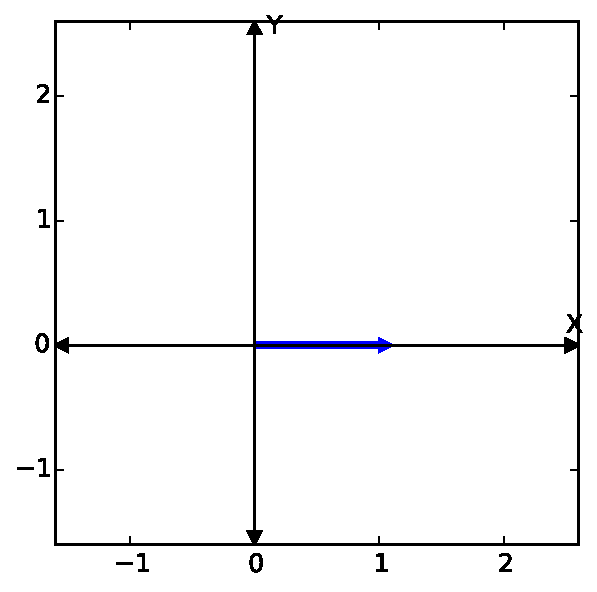
\includegraphics[width=0.46\textwidth]{2DFlipXEig1.pdf}
	}
	\uncover<2->{
	\subfloat[After]{
	    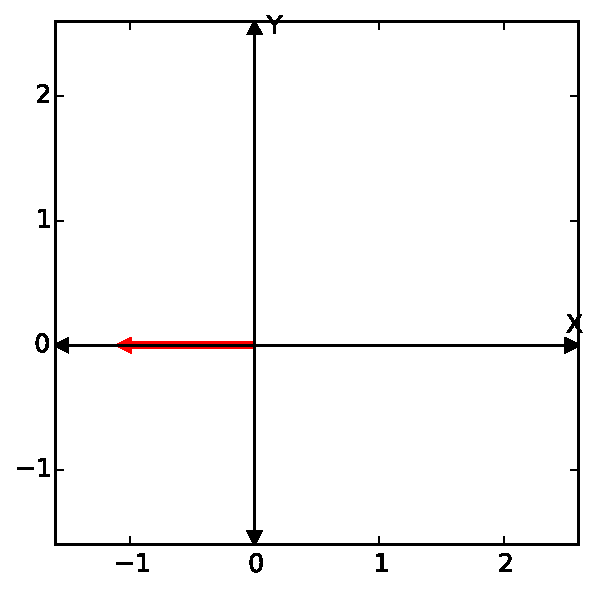
\includegraphics[width=0.46\textwidth]{2DFlipXEig1_T.pdf}
	}
	}
\end{figure}



\end{frame}


\begin{frame}{Eigenvalues/Eigenvectors Example: Flip X, Scale Y}

\only<1>{
\[ \left[ \begin{array}{cc} -1 & 0\\ 0 & 2 \end{array} \right] \left[ \begin{array}{c} 0 \\ 1 \end{array} \right] =   \]
}
\only<2>{
\[ \left[ \begin{array}{cc} -1 & 0\\ 0 & 2 \end{array} \right] \left[ \begin{array}{c} 0 \\ 1 \end{array} \right] =  \left[ \begin{array}{c} 0 \\ 2 \end{array} \right] \]
}

\only<2>{
Yes!  $\lambda = 2$
}

\begin{figure}[t]
    \captionsetup[subfloat]{labelformat=empty}
	\centering
	\subfloat[Before]{
	    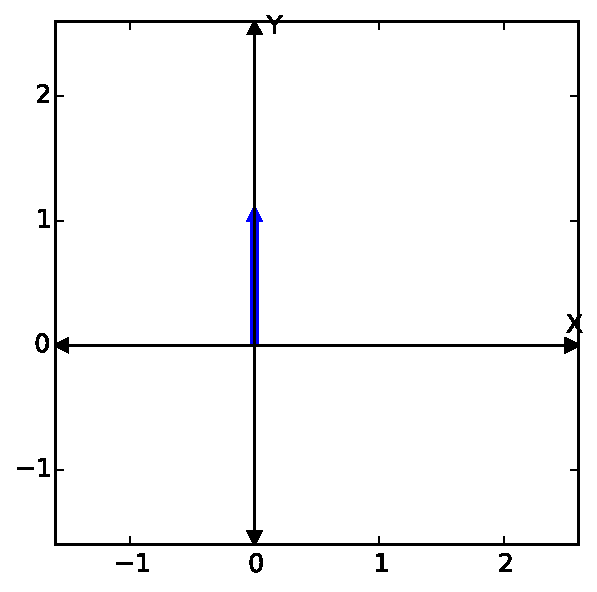
\includegraphics[width=0.46\textwidth]{2DFlipXEig3.pdf}
	}
	\uncover<2->{
	\subfloat[After]{
	    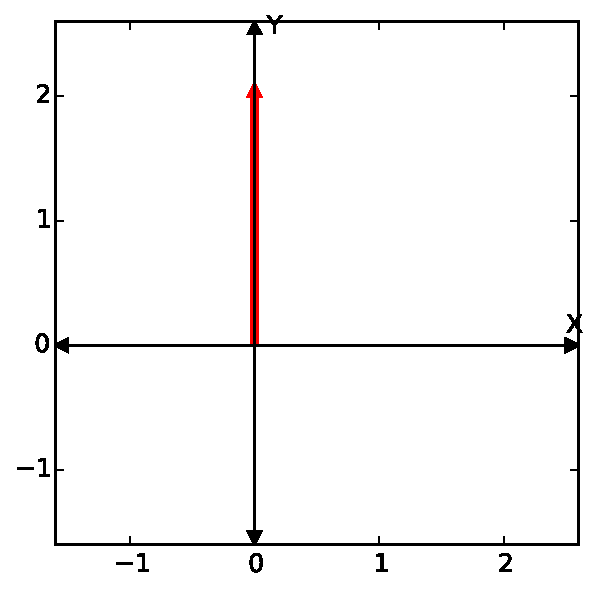
\includegraphics[width=0.46\textwidth]{2DFlipXEig3_T.pdf}
	}
	}
\end{figure}



\end{frame}



\begin{frame}{Eigenvalues/Eigenvectors Example: Flip X, Scale Y}

\only<1>{
\[ \left[ \begin{array}{cc} -1 & 0\\ 0 & 2 \end{array} \right] \left[ \begin{array}{c} 1 \\ 1 \end{array} \right] =   \]
}
\only<2>{
\[ \left[ \begin{array}{cc} -1 & 0\\ 0 & 2 \end{array} \right] \left[ \begin{array}{c} 1 \\ 1 \end{array} \right] =  \left[ \begin{array}{c} -1 \\ 2 \end{array} \right] \]
}

\only<2>{
No, changes direction
}

\begin{figure}[t]
    \captionsetup[subfloat]{labelformat=empty}
	\centering
	\subfloat[Before]{
	    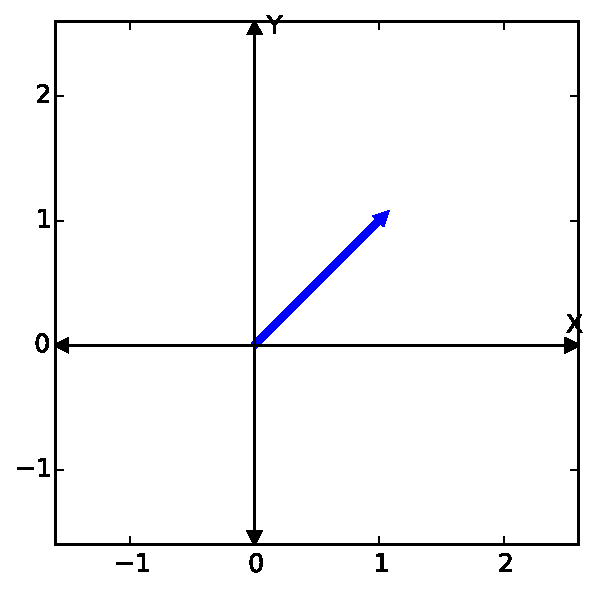
\includegraphics[width=0.46\textwidth]{2DFlipXEig2.pdf}
	}
	\uncover<2->{
	\subfloat[After]{
	    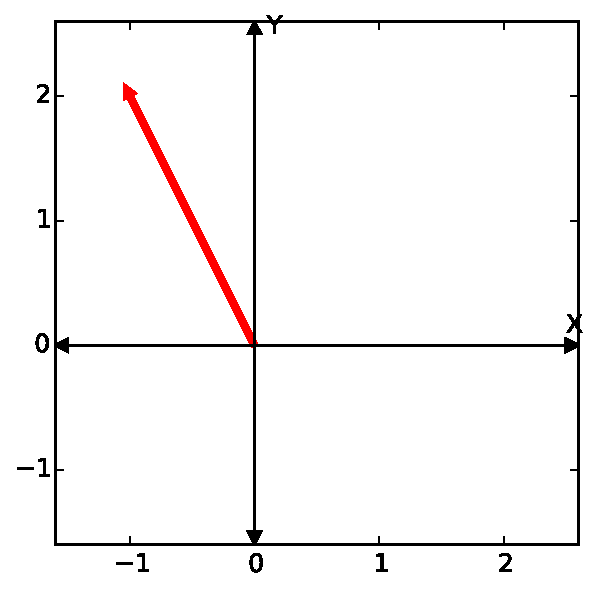
\includegraphics[width=0.46\textwidth]{2DFlipXEig2_T.pdf}
	}
	}
\end{figure}

\end{frame}



\begin{frame}{Rotation Matrix}

What are the eigenvectors/eigenvalues of 

\[ A = \left[ \begin{array}{cc} \cos(\theta) & -\sin(\theta) \\ \sin(\theta) & \cos(\theta) \end{array} \right] \]

?


\end{frame}


\begin{frame}{Linear Eigen-Decomposition}

Eigenvectors/eigenvalues $(\lambda_1, v_1)$, $(\lambda_2, v_2)$

Let 

\[ v = av_1 + bv_2 \]

Then 

\[ Av = A(av_1 + bv_2) = aAv_1 + bAv_2 \]

\[ Av = \lambda_1 a v_1 + \lambda_2 b v_2 \]

\end{frame}


\begin{frame}{Linear Eigen-Decomposition: Example}

\[ \left[ \begin{array}{cc} 4 & -1\\ -1 & 4 \end{array} \right]  \]

\[ v_1 = \left[ \begin{array}{c} -1 \\ -1 \end{array} \right], \lambda_1 = 3\]

\[ v_2 = \left[ \begin{array}{c} -1 \\ 1 \end{array} \right], \lambda_2 = 5 \]

Let $v = \left[ \begin{array}{c}  0 \\ 2 \end{array} \right] $

\end{frame}


\begin{frame}{Spectral Theorem}

If $A$ is {\em symmetric}

\[ \]
 
that is $A = A^T$

\[ \]

then all of its eigenvectors are {\em orthogonal}

\end{frame}



\begin{frame}{Spectral Theorem: Example}


\[ \left[ \begin{array}{cc} 1 & 2\\ 2 & 1 \end{array} \right]  \]


\[ v_1 = \left[ \begin{array}{c} -1 \\ 1 \end{array} \right], \lambda_1 = -1 \]

\[ v_2 = \left[ \begin{array}{c} 1 \\ 1 \end{array} \right], \lambda_2 = 3 \]

\end{frame}


\begin{frame}{Solving for Eigenvalues/Eigenvectors}

\end{frame}


\begin{frame}{Table of Contents}

\begin{itemize}[label=$\vartriangleright$]
	\item Point Clouds Unit Overview
\end{itemize}
\begin{itemize}[label=$\vartriangleright$]
	\item Eigenvalues / Eigenvectors
\end{itemize}
\begin{itemize}[label=$\blacktriangleright$]
	\item Principal Component Analysis
\end{itemize}

\end{frame}


\begin{frame}{Point Cloud Centroid}
Given a collection of points $X = \{\vec{x_i}\}|_{i=1}^N$

Centroid $\vec{c}$ is the ``mean point"

\[ \]

That is

\[ \vec{c}[k] = \frac{1}{N} \sum_{i=1}^N x_i[k] \]

Average each coordinate independently

\end{frame}


\begin{frame}{Point Cloud Centroid}

\begin{figure}[t]
    \centering
	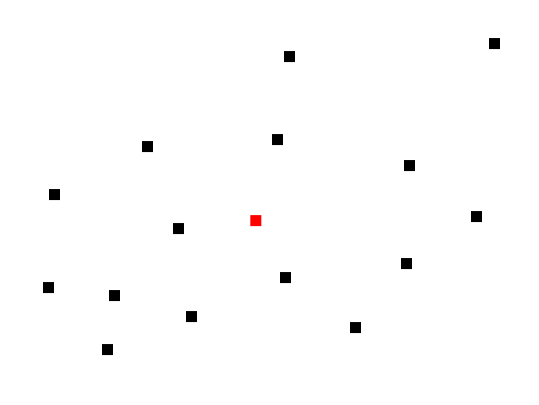
\includegraphics[width=0.9\textwidth]{Centroid1.png}
\end{figure}

\end{frame}


\begin{frame}{Point Cloud Centroid}

\begin{figure}[t]
    \centering
	
\includegraphics[width=0.9\textwidth]{Centroid2.png}
\end{figure}

\end{frame}


\begin{frame}{Directions of Variance}

Organize point cloud into $N \times d$ matrix, each point along a row

\[ X = \left[ \begin{array}{ccc} - & \vec{x_1} & -  \\ - & \vec{x_2} & - \\ - & \vec{x_3} & -  \\ \hdots & \vdots & \hdots \\ - & \vec{x_N} & - \end{array} \right] \]

Choose a unit column vector direction $u \in \mathbb{R}^{d \times 1}$

Then 

\[ d = Xu \]

gives projections onto $u$

\end{frame}


\begin{frame}{Directions of Variance}

\[ d = Xu \]

gives projections onto $u$

\[ \]

\[ d^Td = (Xu)^T(Xu) = u^T (X^TX) u \]

\[ \]

Gives the sum of squared projections onto $u$

\end{frame}


\begin{frame}{Directions of Variance: Example}

1000 point example in 2D, centroid is origin

\begin{figure}[t]
    \centering
	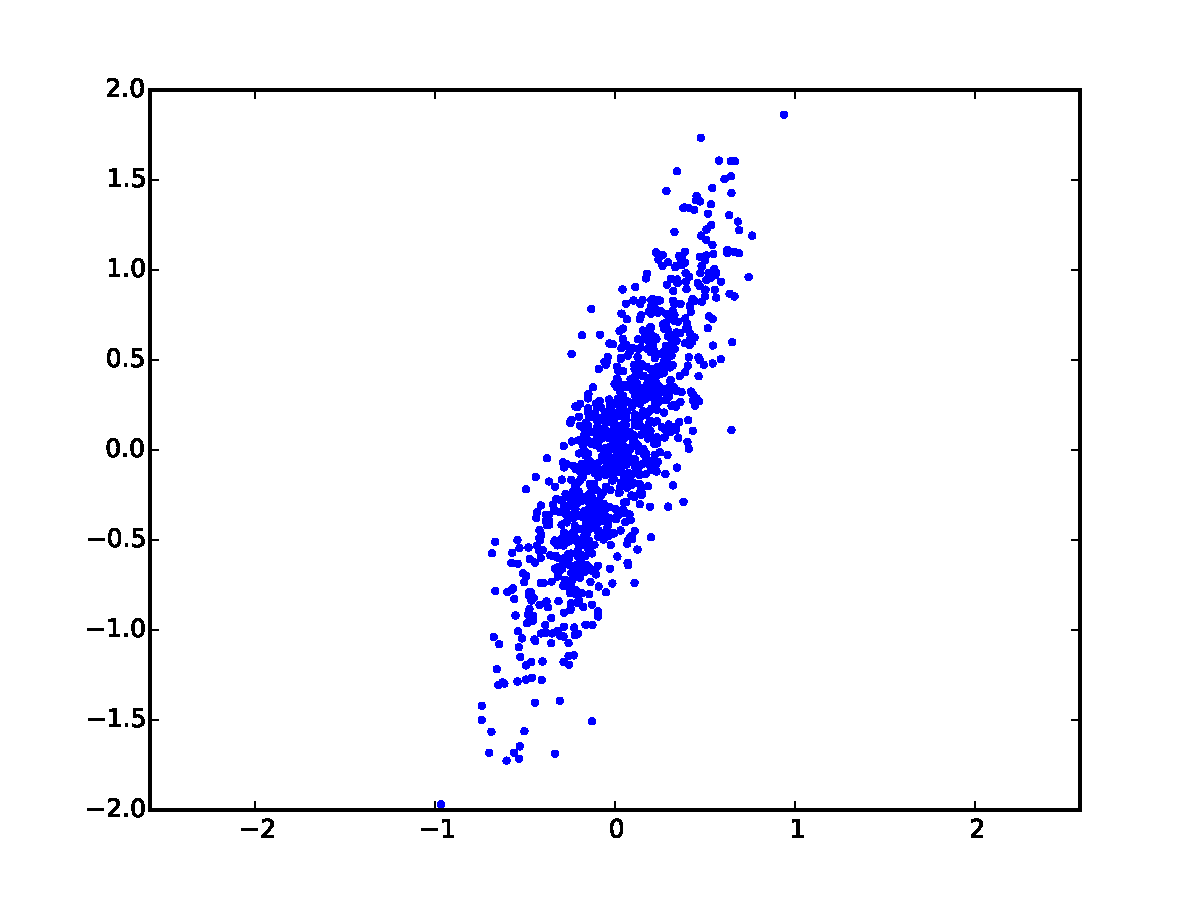
\includegraphics[width=0.9\textwidth]{2DPCAOrig.pdf}
\end{figure}


\end{frame}

\begin{frame}{Directions of Variance: Example}

\begin{figure}[t]
    \centering
	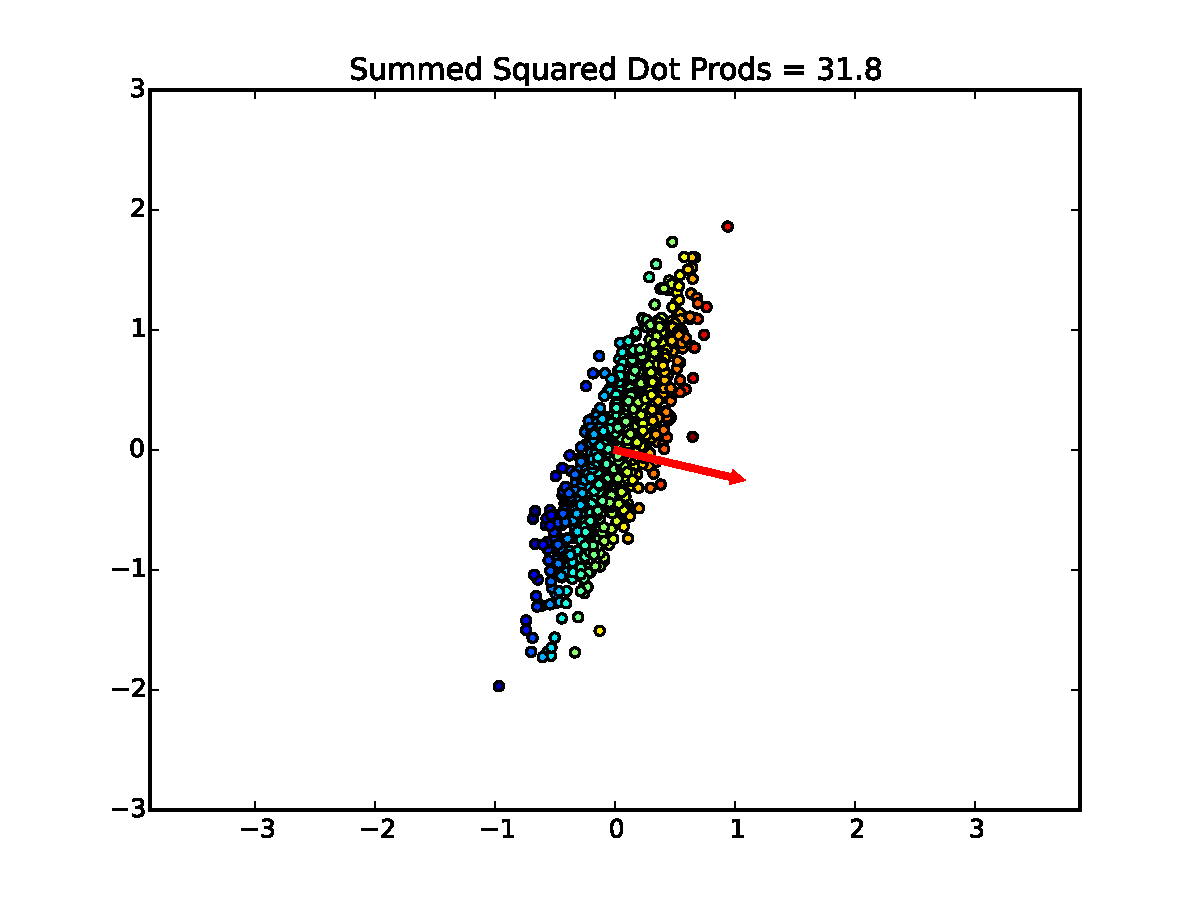
\includegraphics[width=0.9\textwidth]{2DPCADir0.pdf}
\end{figure}

\end{frame}

\begin{frame}{Directions of Variance: Example}

\begin{figure}[t]
    \centering
	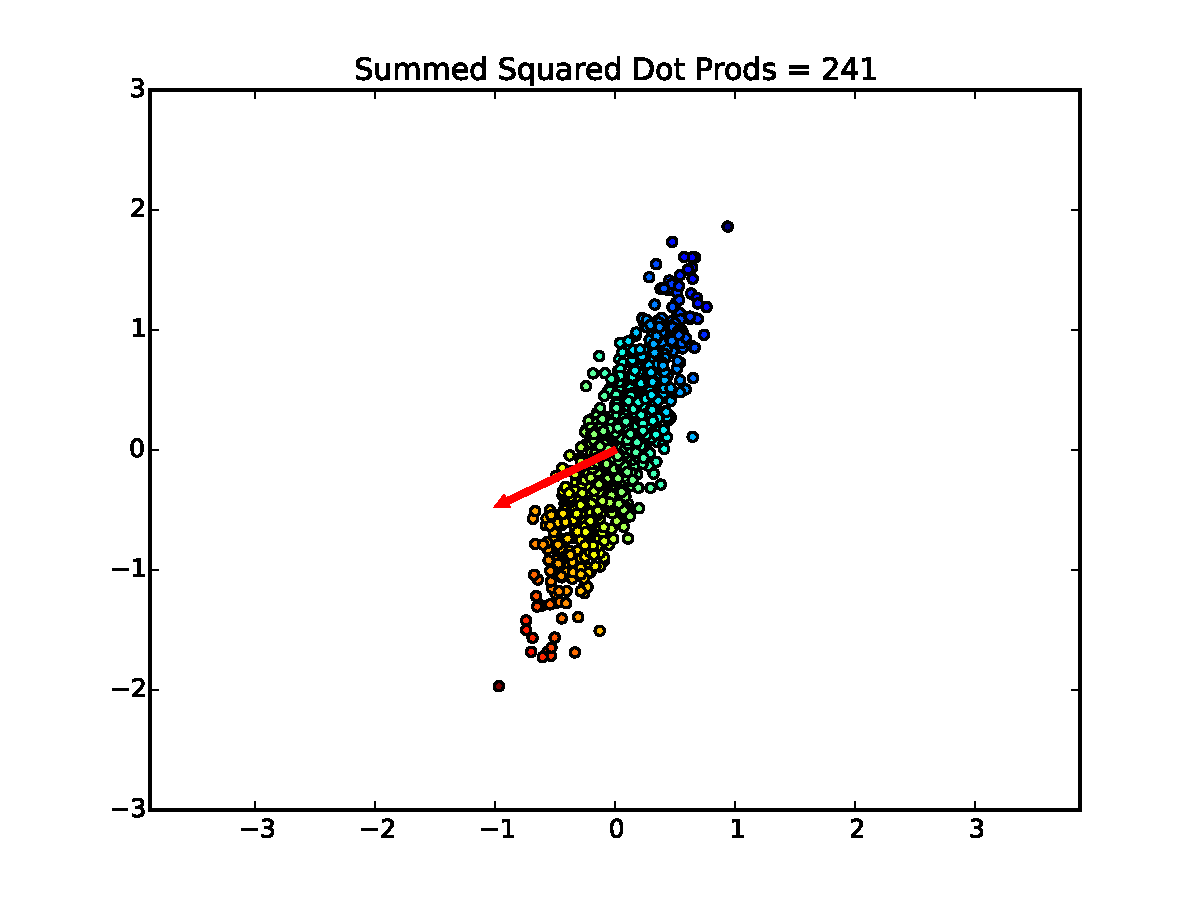
\includegraphics[width=0.9\textwidth]{2DPCADir1.pdf}
\end{figure}

\end{frame}


\begin{frame}{Directions of Variance: Example}

\begin{figure}[t]
    \centering
	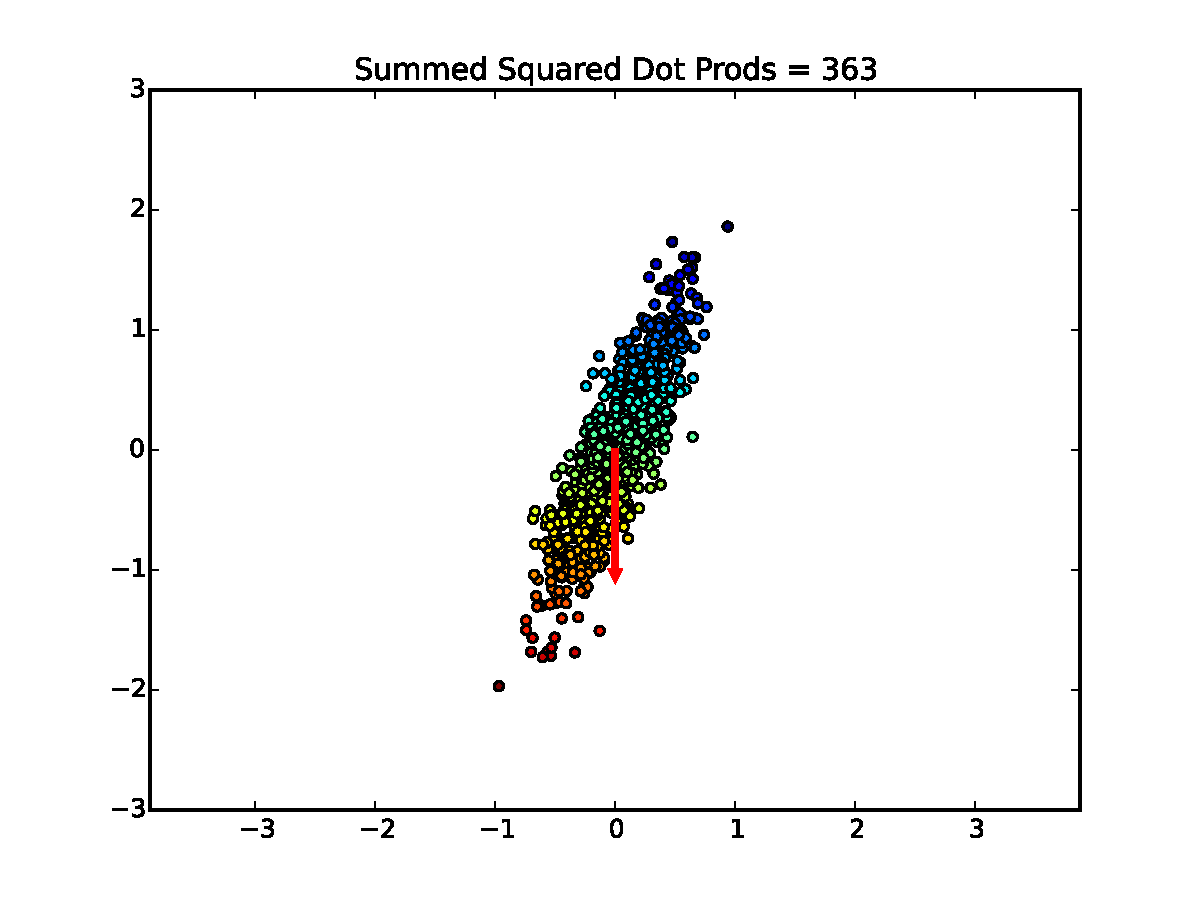
\includegraphics[width=0.9\textwidth]{2DPCADir2.pdf}
\end{figure}

\end{frame}


\begin{frame}{Directions of Variance: Example}

\begin{figure}[t]
    \centering
	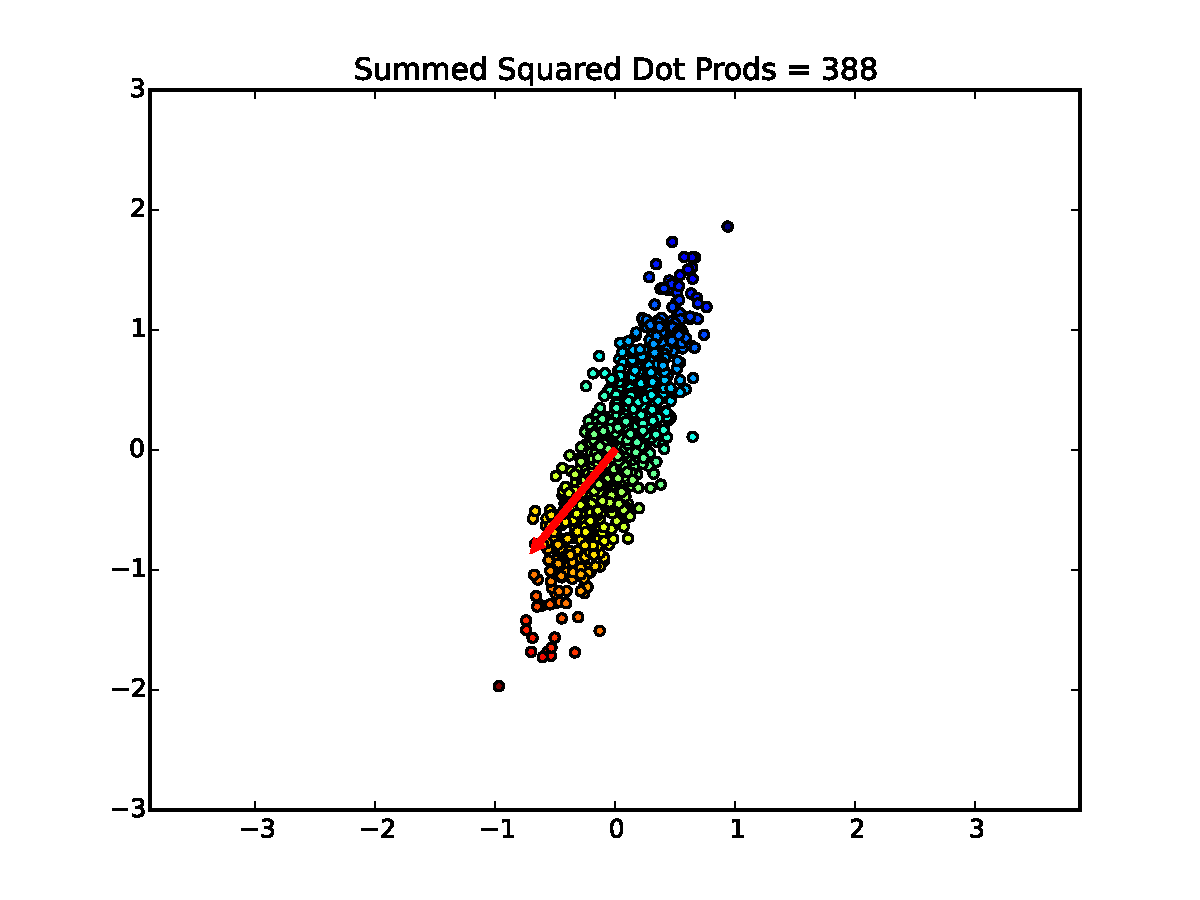
\includegraphics[width=0.9\textwidth]{2DPCADir3.pdf}
\end{figure}

\end{frame}

\begin{frame}{Directions of Variance: Example}

\begin{figure}[t]
    \centering
	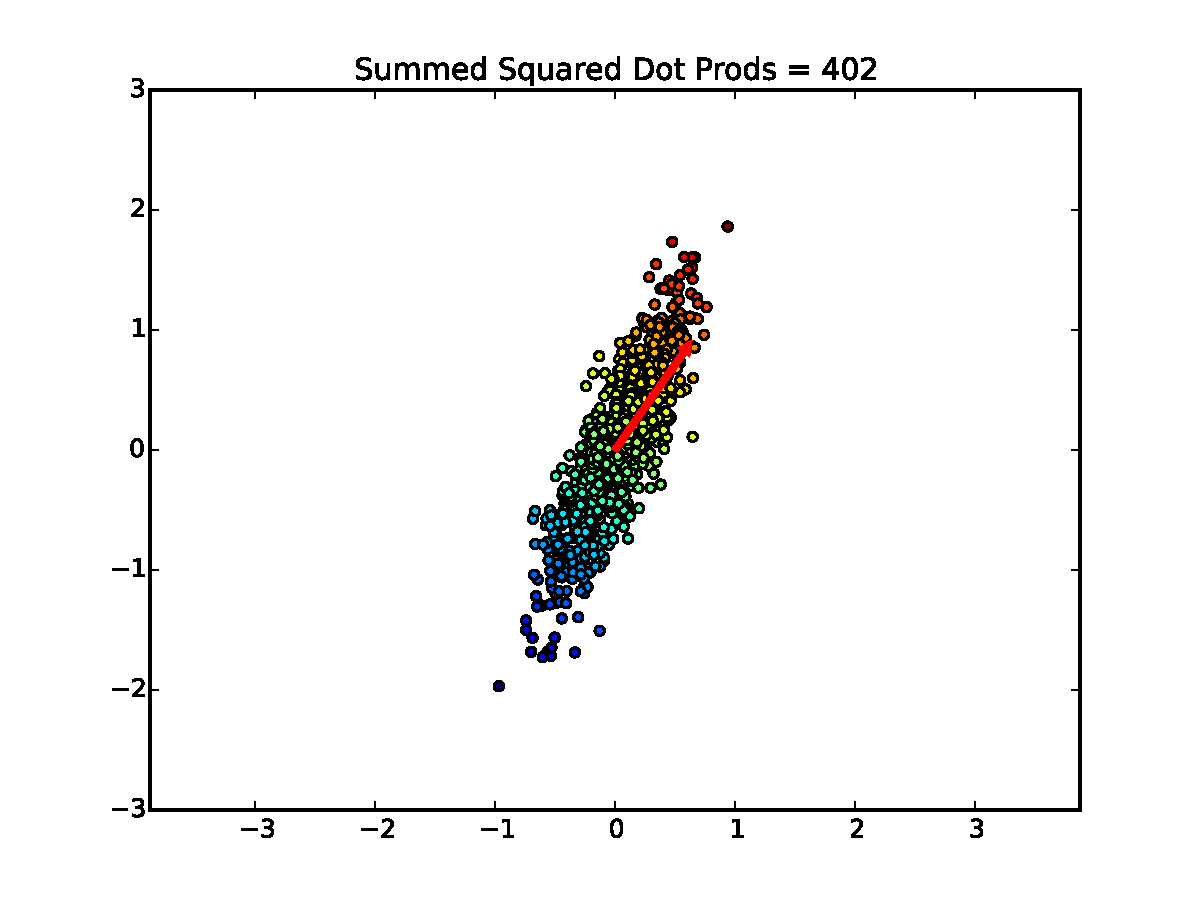
\includegraphics[width=0.9\textwidth]{2DPCADir4.pdf}
\end{figure}

\end{frame}

\begin{frame}{Directions of Variance: Some Math}

\[ d^Td = (Xu)^T(Xu) = u^T (X^TX) u = u^T A u \]

\begin{itemize}[label=$\vartriangleright$]
\uncover<2->{
\item Note that $A = X^TX$ is symmetric.  
}
\uncover<3-> {
\item It is also {\em positive semi-definite}.  All eigenvalues are real and positive
}
\uncover<4-> {
\item
Let $(v_1, \lambda_1)$, $(v_2, \lambda_2)$, ..., $(v_d, \lambda_d)$ be the $d$ eigenvalue/eigenvector pairs.  Then a direction $u$ can be written as

\[ u = a_1 v_1 + a_2 v_2 + \hdots + a_d v_d \]

}

\end{itemize}

\end{frame}

\begin{frame}{Directions of Variance: Some Math}

\[ u^T (X^TX) u = u^T A u \]

Let  $u = a_1 v_1 + a_2 v_2 + \hdots + a_d v_d$

and all $v$s are unit-norm eigenvectors

\uncover<2->{
Then 
\[ u^T A u = (a_1 v_1 + a_2 v_2 + \hdots + a_d v_d)^T A (a_1 v_1 + a_2 v_2 + \hdots + a_d v_d) \]
}

\uncover<3->{
\[ u^T A u = (a_1 v_1 + a_2 v_2 + \hdots + a_d v_d)^T (a_1 \lambda_1 v_1 + a_2 \lambda_2 v_2 + \hdots + a_d \lambda_d v_d) \]
}

\uncover<4->{
Remembering that all $v$s are orthogonal
}

\uncover<5->{
\[ u^T Au = a_1^2 \lambda_1 + a_2^2 \lambda_2 + \hdots + a_d^2 \lambda_d \]
}

\end{frame}


\begin{frame}{Directions of Variance: Some Math}

\[ u^T Au = a_1^2 \lambda_1 + a_2^2 \lambda_2 + \hdots + a_d^2 \lambda_d \]

Assuming that $||u|| = 1 \implies (a_1^2 + a_2^2 + \hdots a_d^2) = 1$

\[ \]

Also assume that $\lambda_1 > \lambda_2 > \hdots > \lambda_d$

\[ \]

Raffle Point Question: What should the $a$s be to maximize the sum of squared dot products: $u^T Au$ ?

\end{frame}

\begin{frame}{Principal Component Analysis}

\begin{itemize}
\item 1. Stack points in rows. 
\item 2. Compute the ``covariance matrix" $A = X^T X$
\item 3. Compute eigenvalues/eigenvectors of $A$, sorted in decreasing order
\item Orthogonal directions of variance are in the eigenvectors
\item Sum of squared dot products with directions are associated eigenvalues
\end{itemize}

\end{frame}

\begin{frame}{PCA Example}

Largest direction of variance, $\lambda_1 = 422$

\begin{figure}[t]
    \centering
	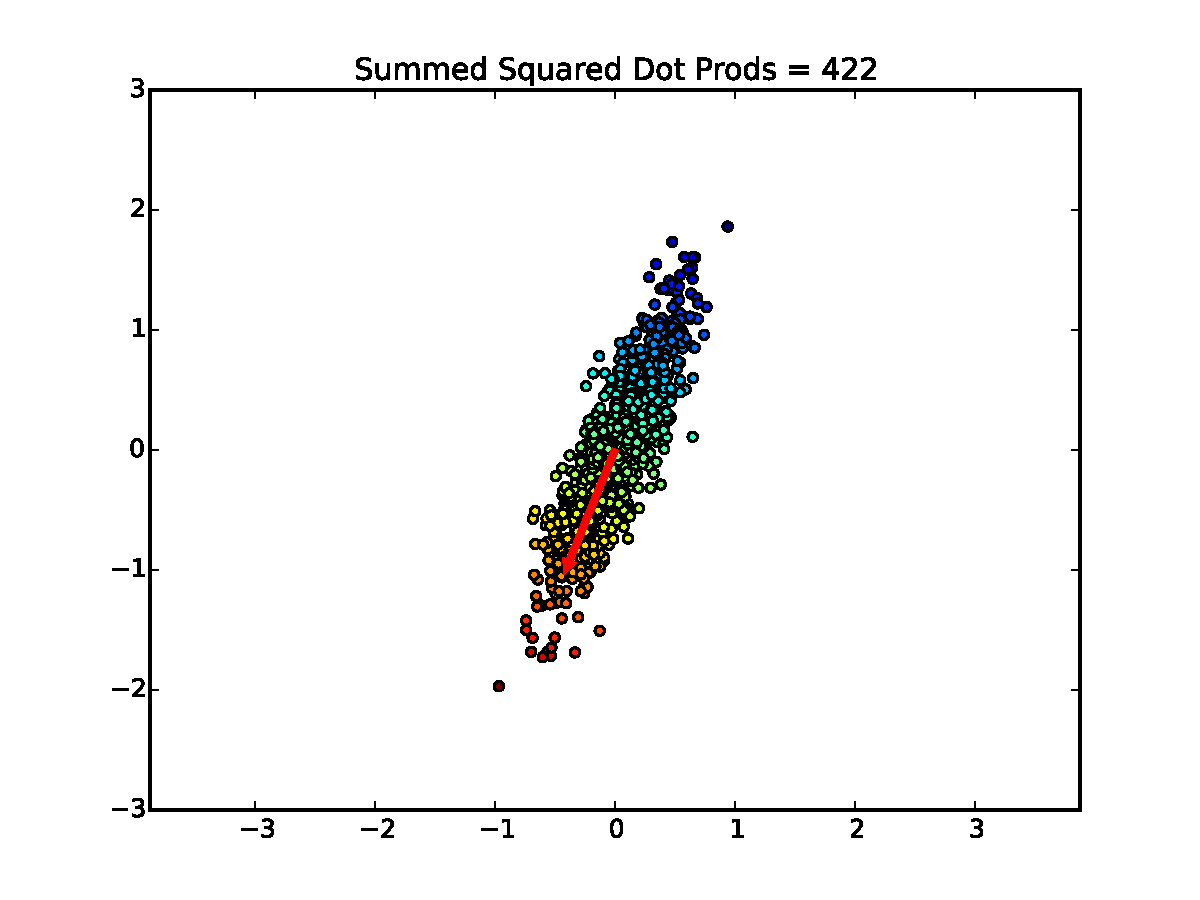
\includegraphics[width=0.9\textwidth]{2DPCADir6.pdf}
\end{figure}


\end{frame}

\begin{frame}{PCA Example}

Smallest direction of variance, $\lambda_2 = 21.6$

\begin{figure}[t]
    \centering
	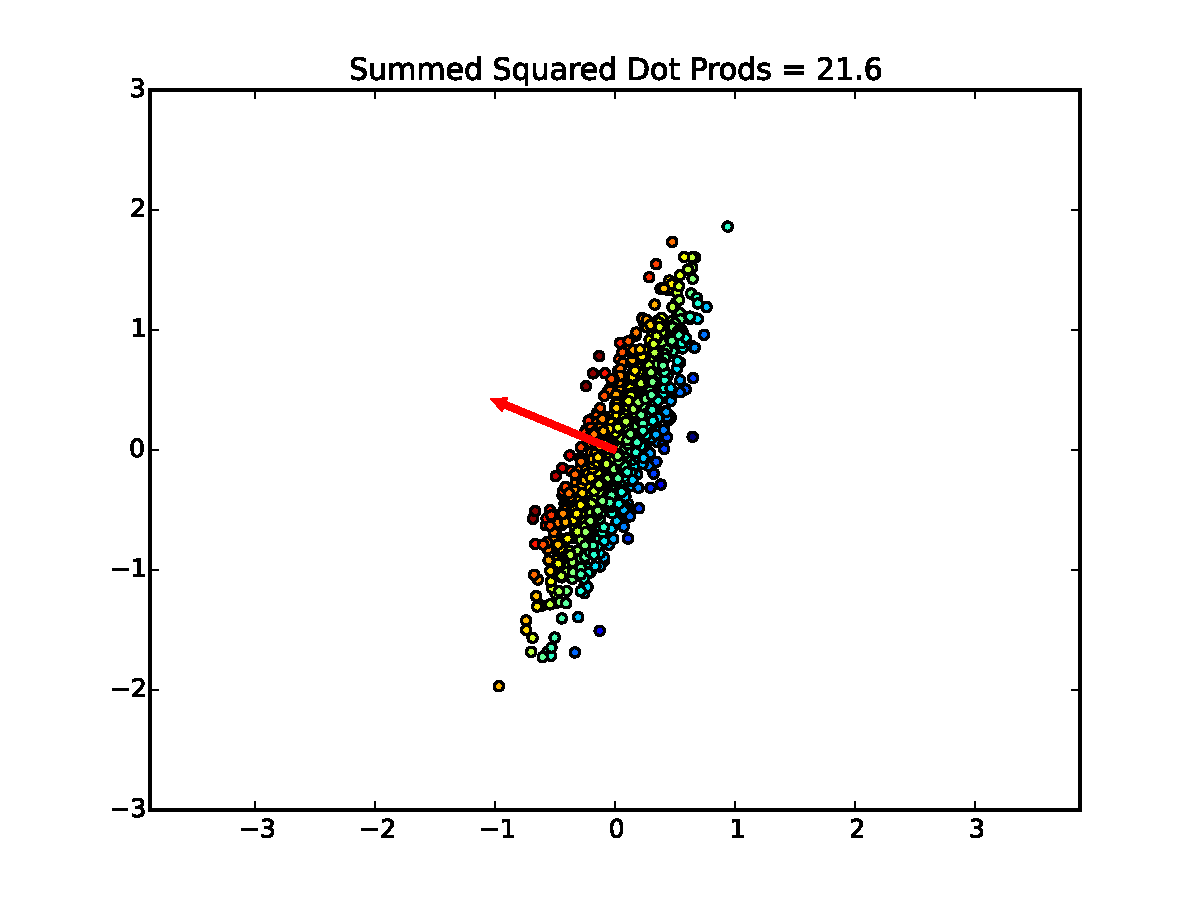
\includegraphics[width=0.9\textwidth]{2DPCADir5.pdf}
\end{figure}


\end{frame}


\begin{frame}{PCA: Interactive Examples 2D/3D}

\end{frame}


\begin{frame}{PCA Pitfalls}

Outliers!

(Show Demo Again)
\end{frame}


\begin{frame}{PCA Pitfalls}


Close Eigenvectors

``Multiplicity issues" for ``near-isotropic" point clouds


\end{frame}

\end{document}

